\chapter{Descrizione del Progetto}
\label{cap:descrizione}

\textit{\indent Questo capitolo fornisce il background tecnico essenziale per comprendere il progetto, analizza le problematiche delle tecnologie coinvolte e illustra l'idea fondamentale alla base del lavoro svolto.}

\section{Background}

~\\
\indent Questa sezione illustra il funzionamento e i principi fondamentali delle tecnologie chiave del progetto.
Queste tecnologie costituiscono la base essenziale per la comprensione di questo studio. 

\subsection{Protocolli di Trasporto Tradizionali}
~\\
\indent Nel panorama dei \gls{protocolli di rete}\glsfirstoccur, i \gls{protocolli di trasporto}\glsfirstoccur \emph{TCP} (Transmission Control Protocol) e \emph{UDP} (User Datagram Protocol) hanno svolto e svolgono tutt'ora un ruolo fondamentale sin dalla nascita di Internet.
Questi protocolli sono stati la spina dorsale delle comunicazioni per decenni, supportando una vasta gamma di servizi e applicazioni.\\
In particolare \emph{TCP}, con la sua affidabilità e il suo controllo di flusso, ha svolto un ruolo fondamentale nelle comunicazioni che richiedevano l'integrità dei dati, mentre \emph{UDP} ha trovato il suo spazio nei servizi che privilegiavano la velocità rispetto all'affidabilità. 
Tuttavia, con l'evoluzione delle nuove tecnologie e la creazione di nuovi protocolli, le limitazioni di questi protocolli sono diventate sempre più evidenti. Nella concezione di base di \emph{TCP} e \emph{UDP}, ideata agli inizi del 1970, non erano state previste le sfide delle reti moderne, 
caratterizzate da :  
\begin{itemize}
    \item Connesioni mobili e variabili;
    
    \item Necessità di ridurre la latenza per la numerosità di applicazione in tempo reale;
    
    \item Proliferazione di dispositivi IOT;
     
    \item Requisiti di sicurezza sempre più vincolanti.
\end{itemize}

Queste nuove sfide hanno evidenziato una serie di problematiche nei protocolli. La consapevolezza di questi limiti ha portato alla ricerca di nuove soluzioni, cercando di superare le inefficienze pur mantenendo tutti i punti di forza.
Questi studi hanno portato alla creazione di nuovi protocolli come \emph{QUIC}\glsfirstoccur ed a estensioni come \emph{MPTCP}\glsfirstoccur, che cercano di far fronte alle sfide del mondo moderno offrendo prestaazioni migliori, maggiore sicurezza e flessibilità.
\\
Nelle sezioni successive esamineremo in dettaglio alcune parti di \emph{TCP} e \emph{UDP}, per poi esplorare come \emph{QUIC} e \emph{MPTCP} si propongono di risolvere e superare le inefficienze presenti e le possibili ripercussioni.

\subsubsection{TCP (Transmission Control Protocol)}

~\\
\indent Il \emph{Transmission Control Protocol (TCP)}, come anticipato nella sezione precedente, è uno dei protocolli cardine su cui si basa la comunicazione su Internet. Dato il suo ruolo e la vasta gamma di funzioni che offre, una analisi completa del suo funzionamento e della sua costituzione richiederebbe un'analisi approfondità che va oltre lo scopo di questa tesi. Pertanto, in questa sezione, ci concentreremo solo su alcuni aspetti specifici del TCP che sono fondamentali per la comprensione del nostro studio su \emph{QUIC}. 
In particolare, esamineremo nel dettaglio :
\begin{itemize}
    \item Caratteristiche principali di una connessione \emph{TCP};
    
    \item Il processo di \emph{Handshake} \glsfirstoccur;
    
    \item I metodi utilizzati per garantire la sicurezza dei dati.
\end{itemize}

\subsubsection{ Caratteristiche principali} 
\indent Il \emph{Transmission Control Protocol} si distingue come un protocollo orientato alla connessione. Questa sua caratteristica significa che, prima di qualsiasi scambio di dati, deve essere stabilita una connessione dedicata tra il \emph{client \glsfirstoccur} e l'\emph{host\glsfirstoccur}.
Questa caratteristica è alla base di molte delle sue funzionalità avanzate, tra cui:
\begin{description}
    \item[Affidabilità] Viene utilizzato il meccanismo degli \emph{acknowledgements} \glsfirstoccur per garantire la corretta consegna dei segmenti;

    \item[Controllo di Errore] Implementa un sistema di verifica della integrità dei dati tramite il meccanismo degli \emph{checksum} \glsfirstoccur;
    
    \item[Controllo di Flusso e Congestione] Utilizza il sistema delle \emph{sliding window} \glsfirstoccur per ottimizzare il flusso di dati e diminuire il numero di segmenti ritrasmetti in caso di situazione di congestione.
\end{description}

Queste funzionalità si riflettono sulla struttura stessa di un segmento TCP, come si può vedere nella Figura \ref{fig}. Segue una breve descrizione delle singole sezioni:

\begin{itemize}
\item \textit{\textbf{Source Port - Destination Port}}: Identificano rispettivamente il numero della porta di origine e destinazione .
\item \textit{\textbf{Sequence Number}}: Questo campo è utilizzato per verificare l'integrità dei dati trasmessi, assicurando che eventuali errori possano essere rilevati e gestiti.
\item \textit{\textbf{Acknowledgement Number}}: Indica la dimensione della finestra di ricezione, permettendo il controllo del flusso di dati tra mittente e destinatario, ottimizzando così la trasmissione.
\item \textit{\textbf{Checksum}}: Contiene i dati effettivi da trasmettere.
\item \textit{\textbf{Data}}: Contiene i dati effettivi da trasmettere.
\end{itemize}

\begin{figure}[!h]
\centering
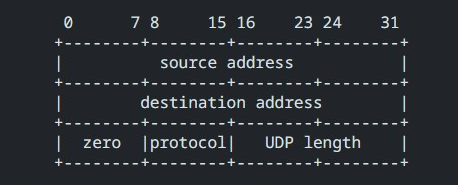
\includegraphics[width=0.8\columnwidth]{descrizione/tcp/segmento}
\caption{Segmento TCP}
\label{fig}
\end{figure}


\paragraph{ Handshake }
\paragraph{ Sicurezza }
\paragraph{ Vantaggi e Svantaggi }
\subsubsection{UDP (User Datagram Protocol)}

\subsection{QUIC}

Spiegazione di quic completa

\subsection{MPTCP}

Spiegazione di quic completa

\section{I problemi e l'Idea}

I problemi di Quic e le nostre idee.

\section{Ispirazione - Related Works ?}

Lavori di Ispirazione, 
